
\documentclass{article}
\usepackage{url}
\usepackage{graphicx}
\usepackage{amsmath}
\usepackage{listings}
\usepackage{float}
\usepackage{xcolor} % for setting colors
\usepackage{color}
\usepackage{CJKutf8}
\usepackage{fancyvrb}


% set the default code style
\lstset{
  frame=tb, % draw a frame at the top and bottom of the code block
  tabsize=4, % tab space width
  showstringspaces=false, % don't mark spaces in strings
  numbers=left, % display line numbers on the left
  commentstyle=\color{green}, % comment color
  keywordstyle=\color{blue}, % keyword color
  stringstyle=\color{red} % string color
}

\definecolor{gray}{rgb}{0.4,0.4,0.4}
\definecolor{darkblue}{rgb}{0.0,0.0,0.6}
\definecolor{cyan}{rgb}{0.0,0.6,0.6}

\lstset{
  basicstyle=\ttfamily,
  columns=fullflexible,
  showstringspaces=false,
  commentstyle=\color{gray}\upshape
}

\lstdefinelanguage{XML}{
  morestring=[b]",
  morestring=[s]{>}{<},
  morecomment=[s]{<?}{?>},
  stringstyle=\color{black},
  identifierstyle=\color{darkblue},
  keywordstyle=\color{cyan},
  morekeywords={xmlns,version,type}% list your attributes here
}

\def\m_space{\vspace{8pt}}

\title{Indri Project Report}
\author{whuang022nccu}
\begin{document}
\maketitle
\section{Introduction}
\subsection{About Indri}
  Indri is a sub version of Lemur project 
  , which is designed for information retrieval and made by C++
  . It contains apis for makeing a customized full-text search engine 
  thst cover such as stemming ,indexing 
  ,scoring the documents and doing the searching.
\subsection{Environment Building}
We prepared a Linux liked environment for the project.
For a cleaning environment to testing and also contains the full GUI system
, we choose to install the virtual machine in the original computer 
which operating system is Ubuntu Desktop 16.04 LTS.

\begin{lstlisting}[language=bash,caption={Install VMware Workstation Player}]
  $ wget https://www.vmware.com/go/getplayer-linux
  $ sudo bash getplayer-linux 
\end{lstlisting}
After the command we will get the installer of vmplayer 
, we just need to run install step by step .

\begin{figure}[H]
  \begin{center}
  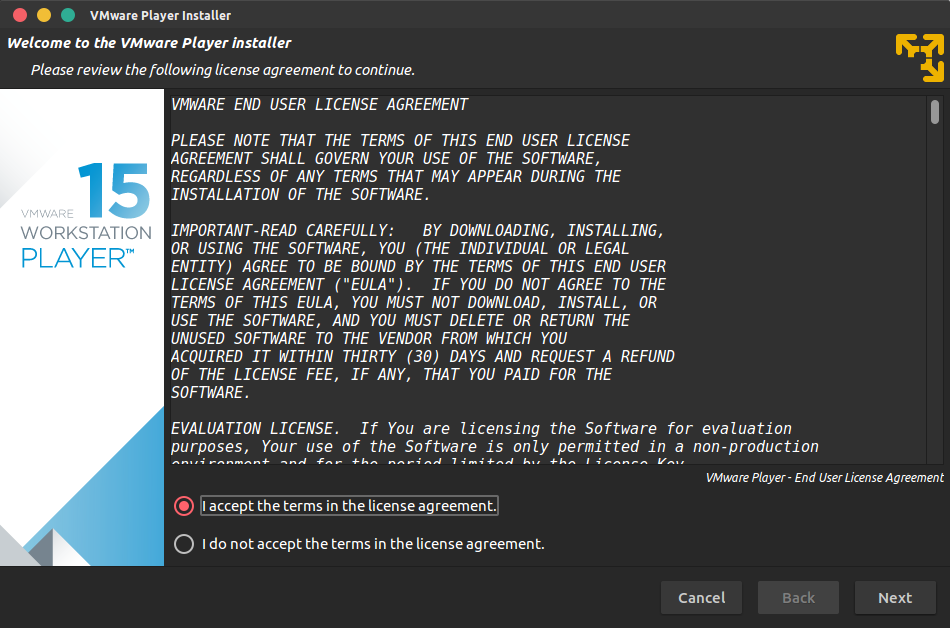
\includegraphics[width=0.5\textwidth]{image/open_the_vmplayer_install.png}
  \caption{Intital Screenshot of vmplayer installer}
  \label{fig:env_01}
  \end{center}
\end{figure}

Next we need the Ubuntu 16.04 ISO file for the vmplayer.

\begin{lstlisting}[language=bash,caption={Get the iso file of Ubuntu 16.04}]
  $ wget http://releases.ubuntu.com/16.04/ubuntu-16.04.6-desktop-amd64.iso
\end{lstlisting}

Now we just need to run the vmplayer and install the Ubuntu.We setting our testing environment called  01\_Ubuntu\_Project\_Indri .
\begin{figure}[H]
  \begin{center}
  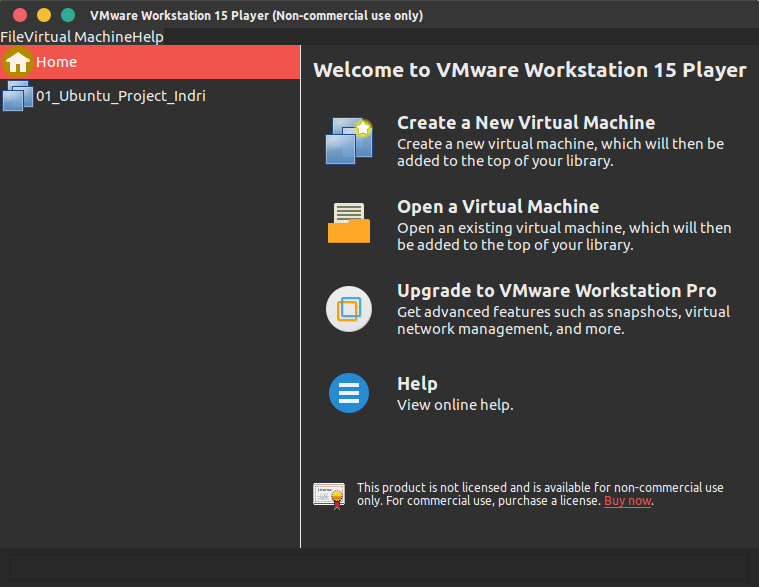
\includegraphics[width=0.5\textwidth]{image/vmplayer_start.png}
  \caption{Intital Screenshot of vmplayer }
  \label{fig:env_02}
  \end{center}
\end{figure}

For checking the system , we can type :

\begin{lstlisting}[language=bash,caption={Get system info}]
  $ sudo apt install inxi 
  $ inxi -M
  $ inxi 
\end{lstlisting}

\begin{figure}[H]
  \begin{center}
  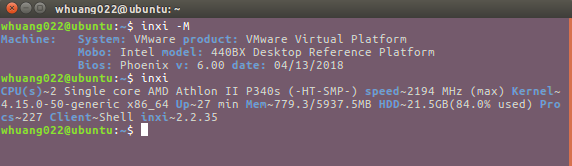
\includegraphics[width=1.0\textwidth]{image/vmplayer_status.png}
  \caption{Checking system info}
  \label{fig:env_03}
  \end{center}
\end{figure}

\subsection{Install Indri}
We get Indri 5.8 :

\begin{lstlisting}[language=bash,caption={Install Indri in bash}]
  $ wget https://sourceforge.net/projects/lemur
  /files/lemur/indri-5.8/indri-5.8.tar.gz/download -O indri-5.8.tar.gz
  $ tar xvfz indri-5.8.tar.gz
\end{lstlisting}
After unzip , we can see the Indri 5.8 folder :

\begin{figure}[H]
  \begin{center}
  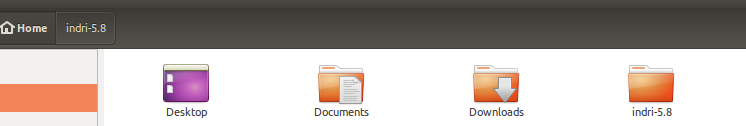
\includegraphics[width=1.0\textwidth]{image/Indri_Folder.png}
  \caption{Checking system info}
  \label{fig:env_04}
  \end{center}
\end{figure}
\m_space
\subsubsection{Installation of dependencies}

There is the list \cite{ref1} that we need to install before compiling the Indri.

\begin{enumerate}
  \item {build-essential:the g++ stuff.}
  \item {git : the version controll system.}
  \item {vim : the bash editor.}
  \item {zlibc :  compressed file-system using in Indri .} 
  \item {zlib1g :  compressed file-system using in Indri .}
  \item {zlib1g-dev :  compressed file-system using in Indri} 
\end{enumerate}
So we just typing : 
\begin{lstlisting}[language=bash,caption={Get dependencies}]
  $ apt-get install build-essential 
  git vim wget zlibc zlib1g zlib1g-dev -y
  $ apt-get update
\end{lstlisting}
For the zlib , we need to change the Makefile \cite{ref2} , and add the compiling flag " -lz " .

\begin{figure}[H]
  \begin{center}
  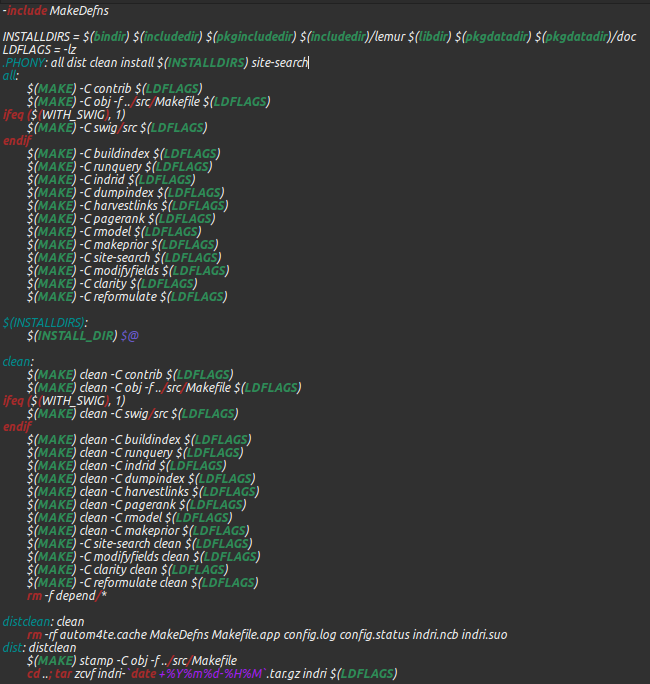
\includegraphics[width=0.8\textwidth]{image/Makefile_edit.png}
  \caption{edit Makefile}
  \label{fig:env_05}
  \end{center}
\end{figure}

\subsubsection{Installation of Indri}
\begin{lstlisting}[language=bash,caption={Install Indri in bash}]
  $ cd ~
  $ cd indri-5.8
  $ sudo ./configure
  $ make
  $ sudo make install
\end{lstlisting}
The system will have Indri after the installation.
\newline\newline\newline\newline\newline
\section{Using Indri to indexing WT2G}

Fist we creat the path of workspace and download the dataset WT2G.And creat the path for indexing.
\begin{lstlisting}[language=bash,caption={ Download WT2G File}]
  $ cd ~
  $ mkdir workspace
  $ cd workspace
  $ wget http://wm5.nccu.edu.tw/base/10001/
  course/10021115/content/proj02/WT2G.tbz
  $ tar jxf WT2G.tbz
  $ mkdir ~/workspace/WT2G_index
  $ mkdir ~/workspace/WT2G_index_no_stemming
  $ mkdir ~/workspace/WT2G_index_parameter_file
  $ mkdir ~/workspace/WT2G_run_shell
\end{lstlisting}
Next we write the  index parameter files ,the format can find at \cite{ref3} .
There will be two types of index file , one is stemming by porter and the other one do not have stemming.
 
\lstset{language=XML}
\begin{lstlisting}[caption={project\_W2T.xml}]
  <parameters>
  <memory>1G</memory>   
  <stemmer>
    <name>porter</name>
  </stemmer> 
  <index>/home/whuang022/workspace/WT2G_index</index>
  <corpus>
    <path>/home/whuang022/workspace/WT2G</path>
    <class>trecweb</class>
  </corpus>
  </parameters>
\end{lstlisting}

\lstset{language=XML}
\begin{lstlisting}[caption={project\_W2T\_withoutstemming.xml}]
  <parameters>
	<memory>1G</memory>   
	<index>/home/whuang022/workspace/WT2G_index_no_stemming</index>
	<corpus>
		<path>/home/whuang022/workspace/WT2G</path>
		<class>trecweb</class>
	</corpus>
</parameters>
\end{lstlisting}
The index parameters files will save at path 

$\sim$/workspace/WT2G\_index\_parameter\_file

\begin{figure}[H]
  \begin{center}
  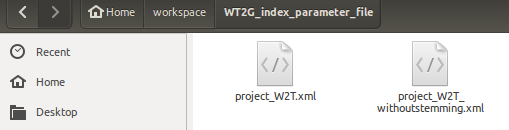
\includegraphics[width=0.8\textwidth]{image/index_par_folder.png}
  \caption{The index parameter files}
  \label{fig:env_06}
  \end{center}
\end{figure}

Then we write shell script to do indexing.We put all shell script in the path 

$\sim$/workspace/WT2G\_run\_shell
\newline\newline
We can use the executable file IndriBuildIndex to build index from bash command .
The command format is IndriBuildIndex $\left[index\_parameter\_file\_path\right]$
\begin{lstlisting}[language=bash,caption={index.sh (use porter stemming)}]

  #!/bin/bash

  cd ~/indri-5.8/buildindex
  
  if [ -e IndriBuildIndex ]
  then
      echo "IndriBuildIndex [OK] "
      ./IndriBuildIndex ~/workspace/WT2G_index_parameter_file
      /project_W2T.xml
  else
      echo "IndriBuildIndex [Error] "
  fi  

\end{lstlisting}


\begin{lstlisting}[language=bash,caption={index\_no\_stemming.sh (no stemming)}]

  #!/bin/bash

  cd ~/indri-5.8/buildindex
  
  if [ -e IndriBuildIndex ]
  then
      echo "IndriBuildIndex [OK] "
      ./IndriBuildIndex ~/workspace/WT2G_index_parameter_file
      /project_W2T_withoutstemming.xml
  else
      echo "IndriBuildIndex [Error] "
  fi
  
  
\end{lstlisting}

\begin{figure}[H]
  \begin{center}
  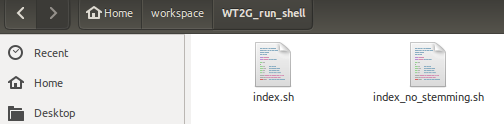
\includegraphics[width=0.8\textwidth]{image/index_sh_folder.png}
  \caption{The index shell scripts }
  \label{fig:env_07}
  \end{center}
\end{figure}

Finally , we just run the shell scripts , ande Indri will generate the index files.


\begin{lstlisting}[language=bash,caption={ Run index shell scripts}]
  $ cd ~/workspace/WT2G_run_shell
  $ sudo bash index.sh
  $ sudo bash index_no_stemming.sh 
\end{lstlisting}
The results is in the index path.
\begin{figure}[H]
  \begin{center}
  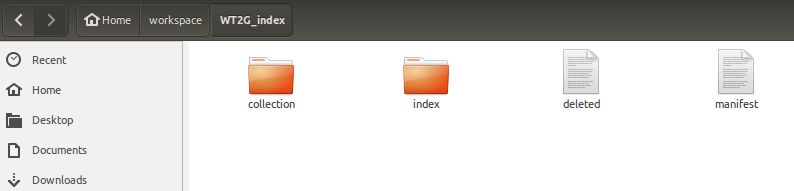
\includegraphics[width=0.8\textwidth]{image/index_out_folder.png}
  \caption{The index files generate from  IndriBuildIndexs }
  \label{fig:env_07}
  \end{center}
\end{figure}

\section{Retrieval Files form Indri index files}
\subsection{Query file and scoring functions}
We can use the executable file IndriRunQuery to doing the retrieval from command ,the scoring can write in the query xml file.The detail information of the format about query file , can read at \cite{ref4}.
The important parameters are:

\begin{enumerate}
  \item { $<$index$>$:the path of index files}
  \item { $<$count$>$ : the number of retun files}
  \item { $<$baseline$>$ : the basic scoring function like Okapi TFIDF }
  \item { $<$method$>$: the other scoring functions }
  \item { $<$query$>$: the query}
\end{enumerate}

\subsubsection{Vector space model Okapi TFIDF}
From the project document there is :
\begin{quotation}
  You will have to use for the weights OKAPI TF x IDF where $ OKAPI TF = tf/(tf + 0.5 + 1.5 * doclen / avgdoclen)$. For queries, Okapi TF can also be computed in the same way, just use the length of the query to replace doclen.
  Also note that the definition of OKAPI TF is$ tf / tf + k1((1 - b) + b * doclen / avgdoclen)$. In the above formula, you can set k1 = 2 and b = 0.75, to end up with:$ tf / (tf + 0.5 + 1.5 * doclen / avgdoclen).$
\end{quotation}
So we just need to set okapi with k1=2.0, b:0.75.
The query file is :

\lstset{language=XML}
\begin{lstlisting}[caption={okapi.xml}]
  <parameters>
	<baseline>okapi,k1=2.0, b:0.75</baseline>  
	<index>/home/whuang022/workspace/WT2G_index</index>
	<count>1000</count>
	<query>
		<type>indri</type>
		<number>401</number>
		<text>
		  foreign minorities germany
		</text>
	</query>
</parameters>
\end{lstlisting}
\subsubsection{Language modeling with Laplace Smoothing}
  Because Indri dose not have an implement of laplace smoothing , so we need to implement the
customized scoring function .In Indri project the scoring functions has an abstract base class named TermScoreFunction.hpp
which was designed for define the scoring function class`s api. 

\begin{figure}[H]
  \begin{center}
  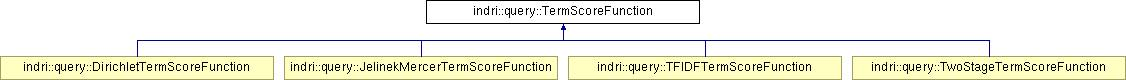
\includegraphics[width=1.0\textwidth]{image/indri_class.jpg}
  \caption{indri::query::TermScoreFunction Class Reference \cite{ref5}}
  \label{fig:env_07}
  \end{center}
\end{figure}

\newpage
\begin{lstlisting}[language=c++,caption={TermScoreFunction.hpp},basicstyle=\tiny]
  #ifndef INDRI_TERMSCOREFUNCTION_HPP
  #define INDRI_TERMSCOREFUNCTION_HPP
  namespace indri
  {
    namespace query
    {
      
      class TermScoreFunction {
      public:
        virtual double scoreOccurrence( double occurrences, int contextLength ) = 0;
        virtual double scoreOccurrence( double occurrences, int contextLength, double documentOccurrences, int documentLength ) = 0;
      };
    }
  }
  #endif // INDRI_TERMSCOREFUNCTION_HPP
\end{lstlisting}
\m_space
  For the customized scoring function , the basic design for the class that extends TermScoreFunction 
is implement the first function "scoreOccurrence( double occurrences, int contextLength )" , and return the first function`s result in the second function.
The laplace smoothing mathod is as the following :$p_i = \frac{m_i+1}{n+k}$where m = term frequency, n=number of terms in document (doc length) , k=number of unique terms in corpus.
In this implementation , we use log transform for $p_i$ to $log\left(p_i\right)$.
The "occurrences" is term frequency , the "contextLength" is number of terms in document.However,we need the size of unique terms in corpus.
So we need to use QueryEnvironment.hpp and it`s api termCountUnique () to get k.The following is the code :

\begin{lstlisting}[language=c++,caption={LaplaceTermScoreFunction.hpp},basicstyle=\footnotesize]

#ifndef INDRI_LAPLACETERMSCOREFUNCTION_HPP
#define INDRI_LAPLACETERMSCOREFUNCTION_HPP
#include <indri/QueryEnvironment.hpp>
#include <math.h>
#include <iostream>
namespace indri
{
  namespace query
  {
    class LaplaceTermScoreFunction : public TermScoreFunction {
    private:
      double _alpha;
      indri::api::QueryEnvironment *env;
    public:
      LaplaceTermScoreFunction(double alpha , const std::string& indexName) {
        _alpha = alpha;
	      env = new indri::api::QueryEnvironment(); 
	      env->addIndex(indexName);
      }
      double scoreOccurrence( double occurrences, int contextSize ) {
        double seen = ( double(occurrences) + _alpha ) / ( double(contextSize) + double(env->termCountUnique ()) );
        return log( seen );
      }
      double scoreOccurrence( double occurrences, int contextSize, double documentOccurrences, int documentLength ) {
         return scoreOccurrence( occurrences, contextSize );
      }
    };
  }
}

#endif // INDRI_LAPLACETERMSCOREFUNCTION_HPP
\end{lstlisting}

To add this customized class to Indri wheile calling the IndriRunQuery , we need to add 
the mapping function in src/TermScoreFunctionFactory.cpp .We add the rule to calling our laplace class :


\begin{lstlisting}[language=c++,caption={TermScoreFunctionFactory.cpp},basicstyle=\footnotesize]

... (some other codes )
else if ( method == "laplace" || method == "l" || method == "lap" ){
    // laplace -- takes parameter "alpha" & index path
    double alpha = spec.get( "alpha", 1.0 );
    return new indri::query::LaplaceTermScoreFunction(alpha,spec.get( "index", "" )); 
  }
... (some other codes )

\end{lstlisting}

Finally , we need to re compile the code (use "make" and "sudo make install") , the new executable file will contain 
the customized api design by us ,and the query file is :

\lstset{language=XML}
\begin{lstlisting}[caption={laplace.xml}]
  <parameters>
	<method>laplace,alpha=1.0,index=/home/whuang022/workspace/WT2G_index</method>  
	<index>/home/whuang022/workspace/WT2G_index</index>
	<count>1000</count>
	<query>
		<type>indri</type>
		<number>401</number>
		<text>
		  foreign minorities germany
		</text>
	</query>
</parameters>
\end{lstlisting}

\subsubsection{Jelinek-Mercer smoothing using the corpus}
The formula for Jelinek-Mercer smoothing is :
$
p_i=\lambda P + \left(1-\lambda\right)Q
$
and we select $\lambda=0.8 $.

Therefore , the query file is :

\lstset{language=XML}
\begin{lstlisting}[caption={jelinek\_mercer.xml}]
  <parameters>
	<rule>method:linear,collectionLambda:0.8,documentLambda:0.2</rule> 
	<index>/home/whuang022/workspace/WT2G_index</index>
	<count>1000</count>
	<query>
		<type>indri</type>
		<number>401</number>
		<text>
		  foreign minorities germany
		</text>
	</query>
</parameters>
\end{lstlisting}

\subsubsection{Jelinek-Mercer smoothing add Laplace}

\begin{lstlisting}[language=c++,caption={JelinekMercerTermLaplaceScoreFunction.hpp},basicstyle=\tiny]



  //
  // JelinekMercerTermLaplaceScoreFunction
  #ifndef INDRI_JELINEKMERCERLAPLACETERMSCOREFUNCTION_HPP
  #define INDRI_JELINEKMERCERLAPLACETERMSCOREFUNCTION_HPP
  #include <indri/QueryEnvironment.hpp>
  #include <math.h>
  namespace indri
  {
    /// indri query processing and scoring components.
    namespace query
    {
      
      class JelinekMercerLaplaceTermScoreFunction : public TermScoreFunction {
      private:
        double _lambda;
        double _backgroundLambda;
        double _collectionFrequency;
        double _collectionComponent;
        double _oneLevelCollectionComponent;
        double _contextLambda;
        double _collectionLambda;
        double _documentLambda;
        double _foregroundLambda;
        indri::api::QueryEnvironment *env;
      public:
        JelinekMercerLaplaceTermScoreFunction( double collectionFrequency, double collectionLambda, double documentLambda  , const std::string& indexName ) {
          _contextLambda = (1 - collectionLambda - documentLambda);
          _collectionFrequency = collectionFrequency;
          _collectionLambda = collectionLambda;
          _documentLambda = documentLambda;
          _foregroundLambda = (1 - _collectionLambda);
          env = new indri::api::QueryEnvironment(); 
    env->addIndex(indexName);
  
          assert( _documentLambda >= 0.0 && _documentLambda <= 1.0 );
          assert( _collectionLambda >= 0.0 && _collectionLambda <= 1.0 );
          assert( _contextLambda >= 0.0 && _contextLambda <= 1.0 );
      
          _collectionComponent = _collectionLambda * _collectionFrequency;
        }
  
        double scoreOccurrence( double occurrences, int contextSize ) {
          double seen2 = ( double(occurrences) +1.0 ) / ( double(contextSize) + double(env->termCountUnique ()) );
          double contextFrequency = contextSize ? occurrences / double(contextSize) : 0.0;
          return (log( _foregroundLambda * contextFrequency + _collectionComponent )+log(seen2));
        }
  
        double scoreOccurrence( double occurrences, int contextSize, double documentOccurrences, int documentLength ) {
          double seen2 = ( double(occurrences) +1.0 ) / ( double(contextSize) + double(env->termCountUnique ()) );
          double contextFrequency = contextSize ? occurrences / double(contextSize) : 0.0;
          double documentFrequency = documentLength ? documentOccurrences / double(documentLength) : 0.0;
          return (log( _contextLambda * contextFrequency + _documentLambda * documentFrequency + _collectionComponent )+log(seen2));
        }
      };
    }
  }
  
  #endif // INDRI_JELINEKMERCERLAPLACETERMSCOREFUNCTION_HPP
  
  \end{lstlisting}
\subsection{The shell script to Retreival}
For example of laplace we will have :
\begin{lstlisting}[language=bash,caption={ Run index shell scripts},basicstyle=\tiny]
#!/bin/bash

cd ~/indri-5.8/runquery

if [ -e IndriRunQuery ]
then
    echo "IndriRunQuery [OK] "
    ./IndriRunQuery ~/workspace/WT2G_query_parameter_file/laplace.xml -trecFormat=true > ~/workspace/WT2G_result/output_laplace.txt
    cd ~/workspace/WT2G_result/
    perl trec_eval.pl [-q] qrels.401-450.txt output_laplace.txt > laplace_evaluation.txt
else
    echo "IndriRunQuery [Error] "
fi
\end{lstlisting}


\newpage
\section{Result}

\subsection{Un-interpolated Mean Average Precision}
\begin{table}[htb]
  \begin{tabular}{|l|l|l|l|l|}
    \hline
            & Okapi TF&Laplace&Jelinek Mercer&Jelinek Mercer add Laplace \\
    \hline
   stemming &0.2704&0.5123&0.0591&0.5123\\
   \hline
   no stemming&0.1932&0.3205&0.0407&0.3205\\
   \hline
  \end{tabular}
\end{table}

\subsection{Precision at rank 10 documents}
\begin{table}[htb]
  \begin{tabular}{|l|l|l|l|l|}
    \hline
            & Okapi TF&Laplace&Jelinek Mercer&Jelinek Mercer add Laplace \\
    \hline
   stemming &0.3000&0.9000&0.1000&0.9000\\
   \hline
   no stemming&0.3000&0.8000&0.0000&0.8000\\
   \hline
  \end{tabular}
\end{table}

In conclution , if we do not stemming the performace is not good at all.

\subsection{Access the project}


\begin{lstlisting}[language=bash,caption={Access the project }]

  1. The source code with customized class : 
https://github.com/whuang022nccu/IndriLab 
2. The shell scripts (.sh) , parameter files (.xml) ,and reslut files : 
https://github.com/whuang022nccu/IndriLab/tree/master/parameter%20files%20 
  \end{lstlisting}


\newpage
\begin{thebibliography}{99}  
  \bibitem{ref1}Can't Make - error, \url{https://sourceforge.net/p/lemur/discussion/2106523/thread/3abe18beed/}, 25 04 2019.
  \bibitem{ref2}Compilation problems with ZLIB, \url{https://stackoverflow.com/questions/
  9700414/compilation-problems-with-zlib/18875275#18875275}, 16 03 2012.
  \bibitem{ref3}IndriBuildIndex Parameters, David Fisher , \url{https://sourceforge.net/p/lemur/wiki/IndriBuildIndex%20Parameters/}
  \bibitem{ref4}Specifying Retrieval Parameters, David Fisher , \url{https://sourceforge.net/p/lemur/wiki/IndriRunQuery/}
  \bibitem{ref5}indri::query::TermScoreFunction Class Reference , \url{https://lemur.sourceforge.io/indri/classindri_1_1query_1_1TermScoreFunction.html}

 
\end{thebibliography}
\end{document}

